% coming soon

We have implemented our switching approach in the MAPSIM
environment~\cite{brenner:nebel:jaamas09},
using \system{dlib-ml}~\cite{king:2009} for belief
revision. Sequential sessions use a modified version of Fast
Downward~\cite{fast-downward}, and DT sessions use our own contingent
procedure. Since most of the problems we consider are much larger than
any available DT planner can solve directly, for comparison purposes
we also implemented a simple dual-mode replanning baseline
approach. Here, when a switching action is scheduled for execution the
DT session plans to a single entropy reduction action, whose execution
can provide evidence regarding the truth value of a relevant
assumption.
%%
%%  -- i.e,. we say a fact can
%% be directly sensed, if there is a DTPDDL {\em sense} declaration that
%% mentions the fact in its precondition. 
%%
Control is then immediately
returned to a new sequential session.


We evaluate our approaches in robot exploration tasks from home and
office environments. Spatially, these consist of {\em rooms}
(office/kitchen/etc), and an underlying topological map over
smaller areas of space, called {\em places}, and connectivity between
those. The mobile {\em robot} and {\em visual objects} inhabit the
topological places. Objects indicate the category of space they
inhabit---e.g., spoons are likely to be in kitchens. By examining
view cones at places for particular objects, the robot is able to: (1)
categorise space at high (room) and low (place) levels, and (2) find
objects for the user, exploiting information about object
co-occurrence and room categories for efficiency. Also, in the
presence of a person, the robot can ask about the category of the
current room.


We compare switching to the baseline in several realistic
tasks, with the number of rooms ranging from 3 (12-places, 16-objects,
$|$states$|$ $>10^{21}$) to 6 (26-places, 21-objects, $|$states$|$
$>10^{36}$). We also compare those systems with near optimal policies
computed using Smith's {\sc zmdp} for small 2 room problems (4-places,
3-objects, $|$states$|$ $\simeq 5000$). Our evaluation considers 3
levels of reliability in sensing: {\em reliable} sensors have a $.1$
probability of a false negative, {\em semi-reliable} have a chance of
$0.3$ of false negative and $0.1$ of false positive, and {\em noisy}
sensors with probabilities of $0.5$ and $0.2$ respectively. Each
object class is assigned one sensor model---e.g. cornflakes may be
harder to detect than refrigerators. We performed several experiments
with different levels of reliability for sensing the target object(s),
while keeping sensing models for non-target objects constant.

\Omit{
All non-target objects remain unchanged so the planner can
exploit object co-occurrences using reliably sensed objects to
compensate for the increased sensor noise.
}

Our evaluation examines DT sessions with initial belief-states
admitting between 20 and 100 abstract states with non-zero
probability. We run 50 simulations in each configuration, and have a
timeout on each simulation of 30 minutes (1800 seconds)\footnote{All
experiments were conducted on a 2.66GHz Intel Xeon X5355 using one CPU
core.}. The continual planning times are reported in
Figure~\ref{fig:results-time}, and the quality data in
Figure~\ref{fig:results-quality}.
%%
For each task, the goal is to find one or more objects and report
their position to a user. Usually there is a non-zero probability that
no plan exists, as the desired object might not be present in the
environment.
% MOG: I didn't do  evaluations for those, so let's remove them
% Item~$f$ reports for tasks requiring indirect sensing,
% where the robot must relocate to a room with a particular category
% (e.g. kitchen). the {\em baseline} is not able to complete Item~$f$,
% so is omitted from that reporting.  
In these experiments we only allocate reward on the achievement of all
goals, therefore we find it intuitive to report average plan costs and
the success rates in problems that admit a complete solution (i.e.,
positive reward scaled by a constant factor). The exception occurs for
items f and g of Figure~\ref{fig:results-quality}, where we report
expected discounted rewards (not plan costs).

\begin{figure}[h!]
  % \centering
  % 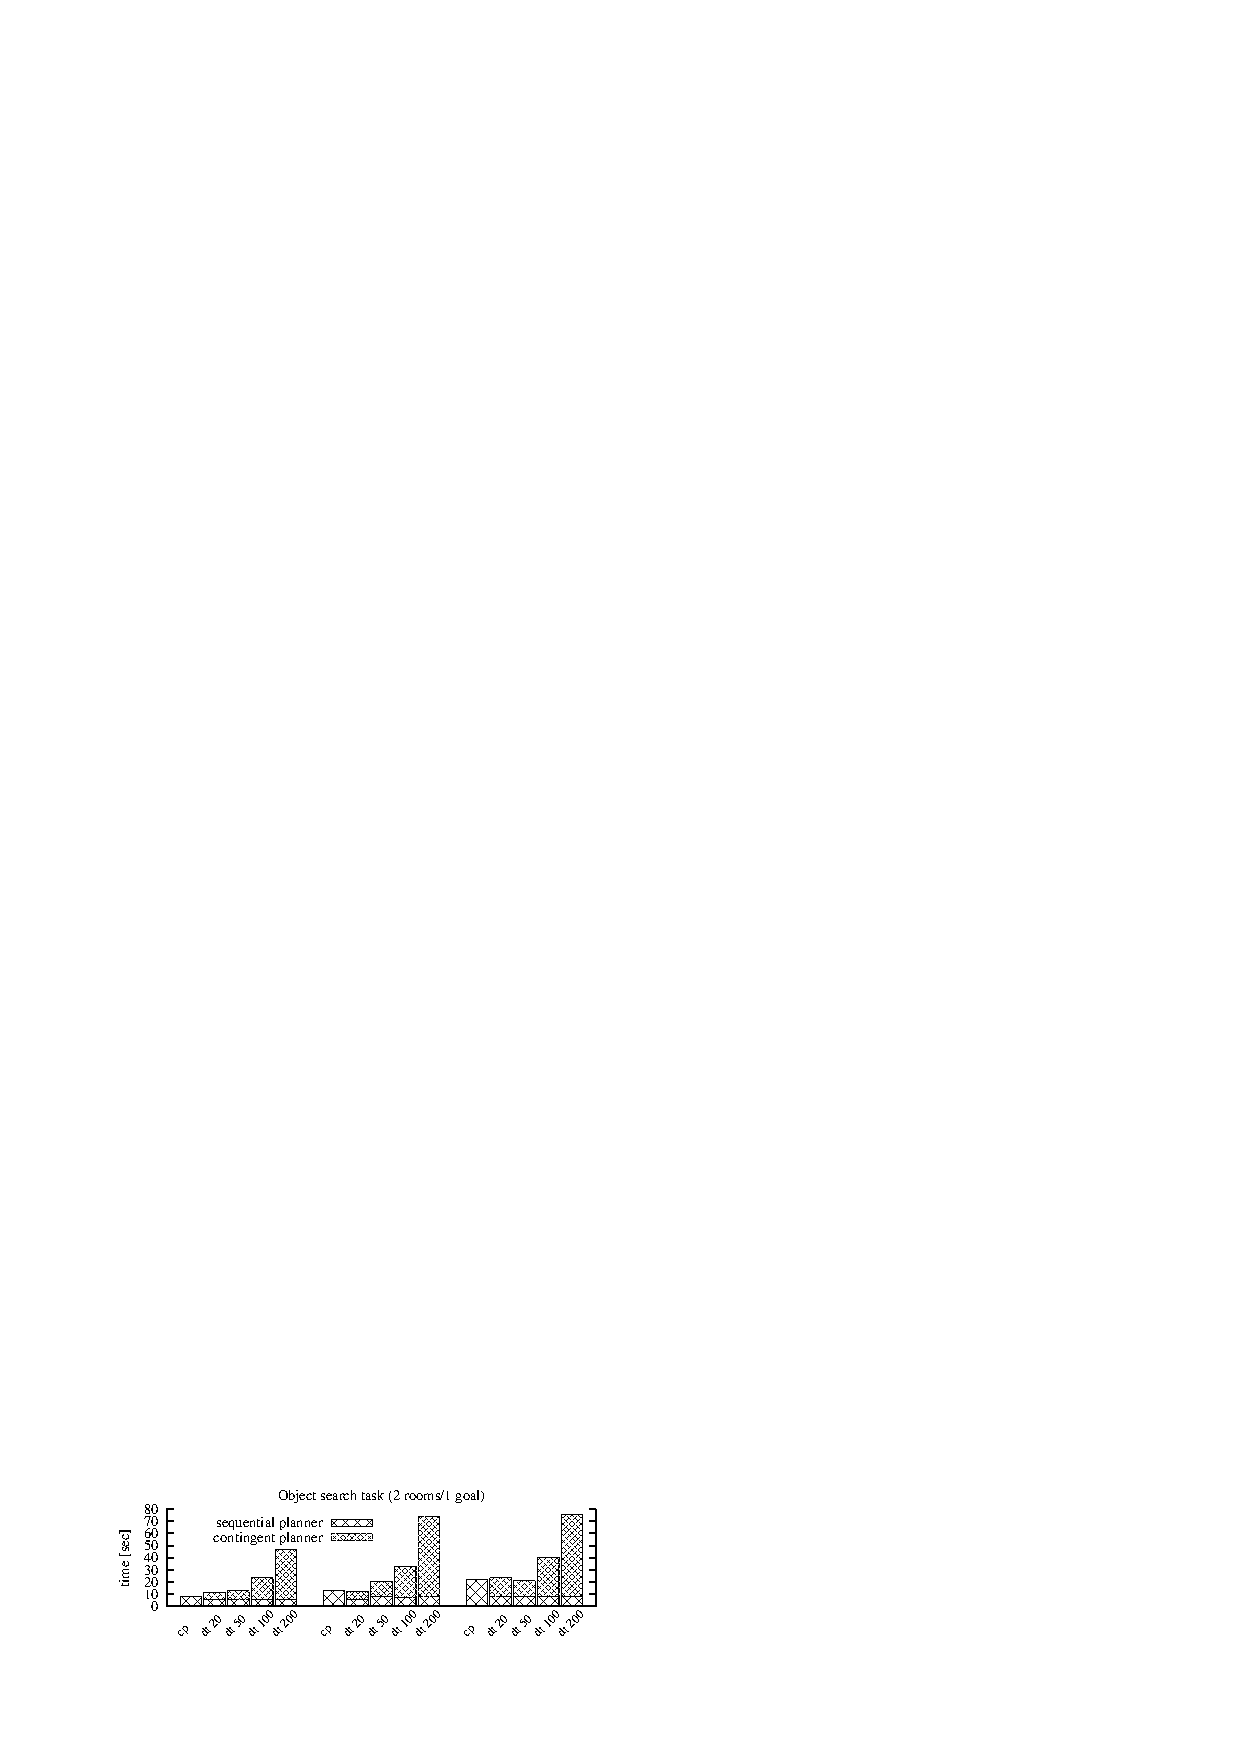
\includegraphics{dora1-time}\hfill
  % \vspace{2mm}
  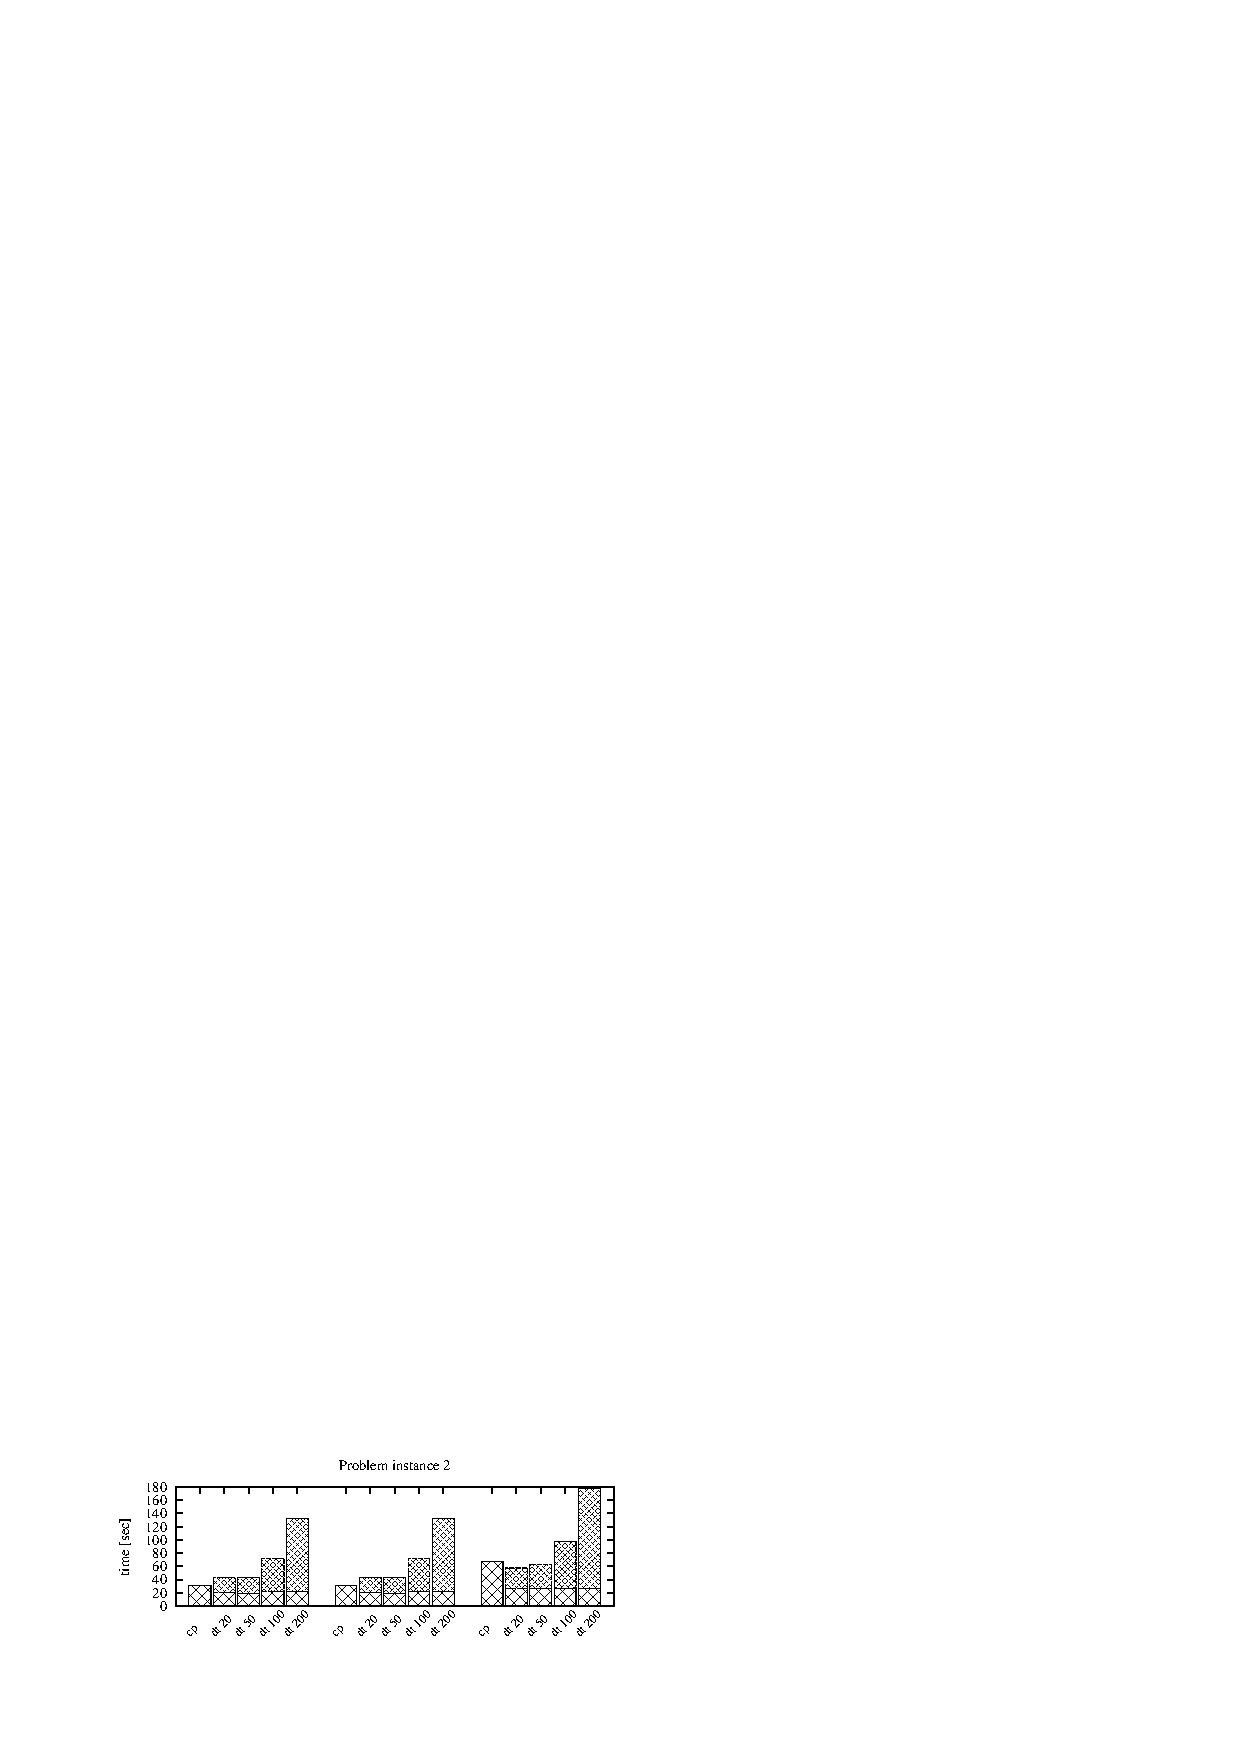
\includegraphics{dora2-time}\hfill
  % \vspace{2mm}
  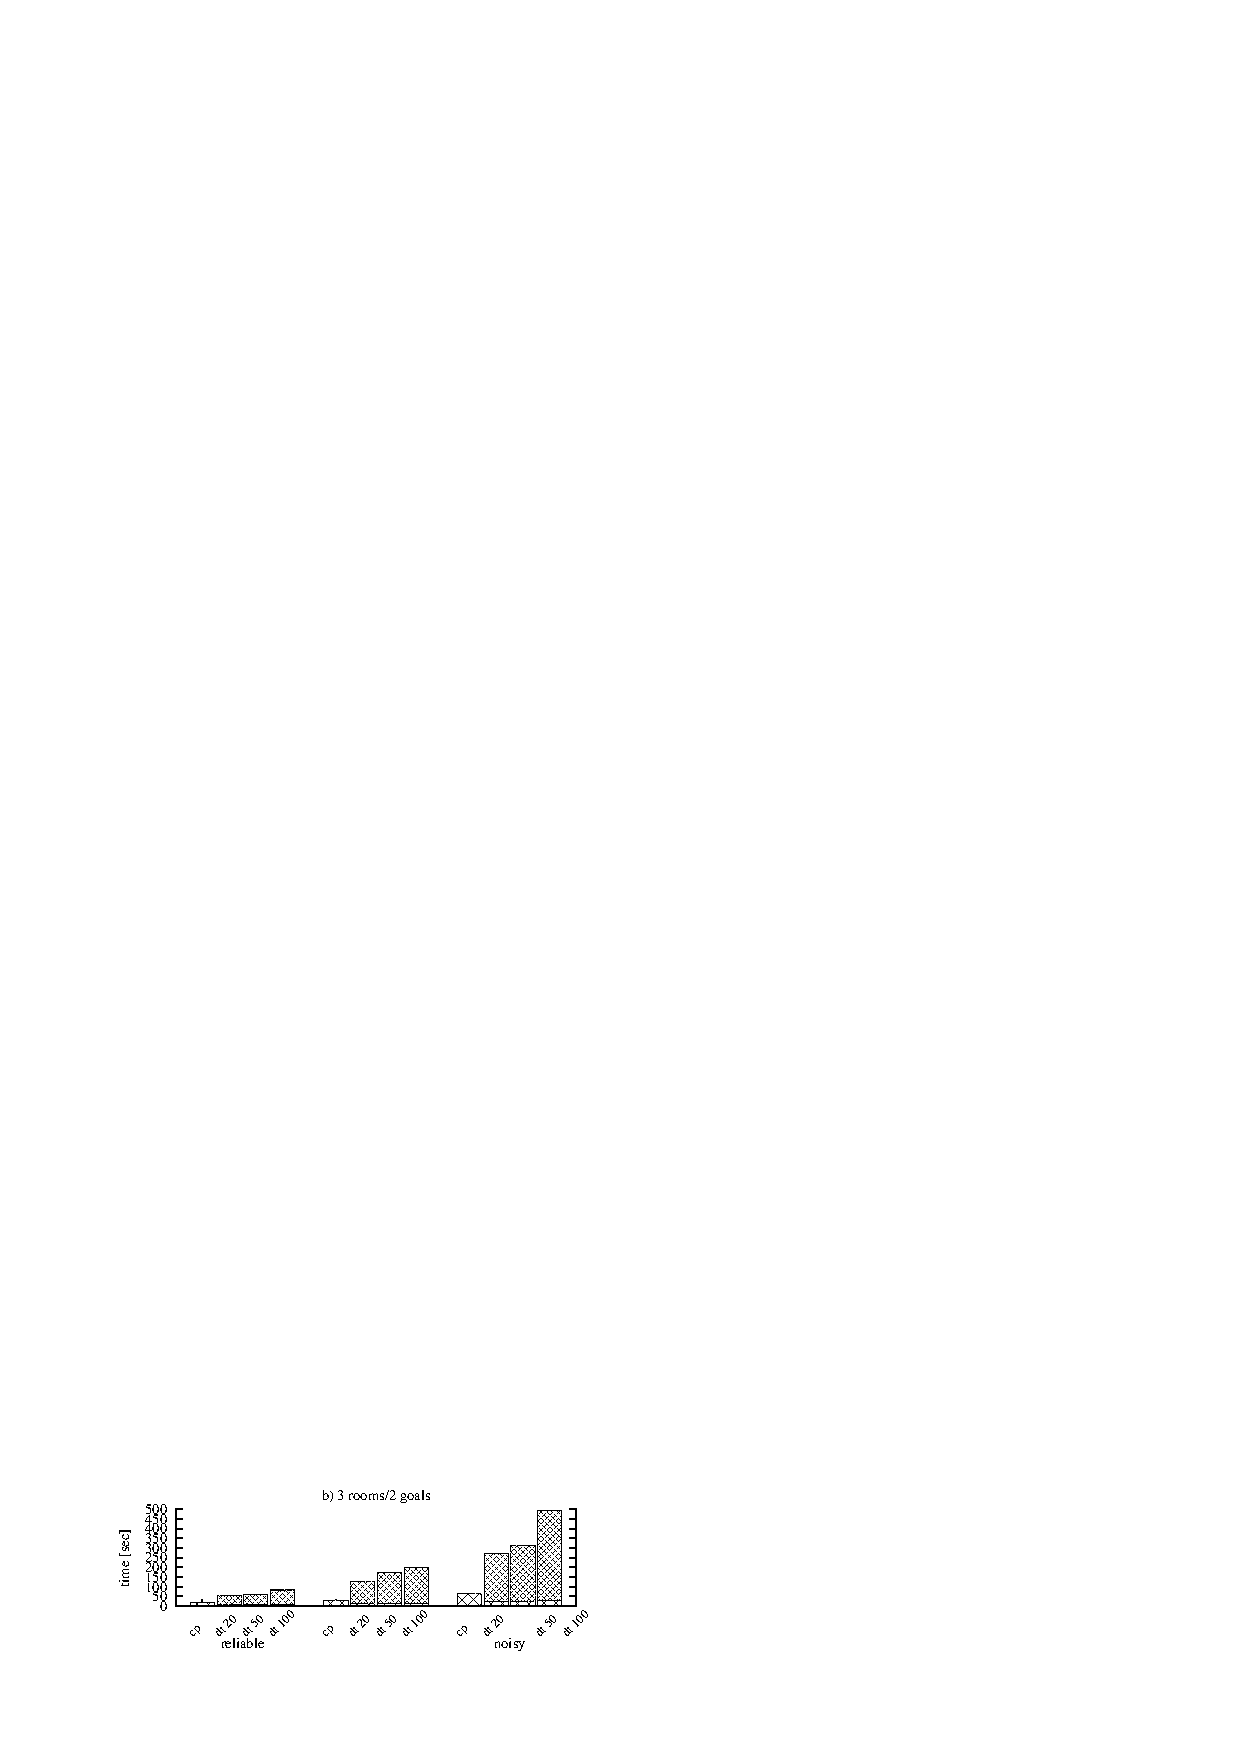
\includegraphics{dora3-time}\hfill
  % \vspace{2mm}
  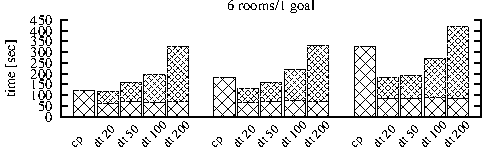
\includegraphics{dora4-time}\hfill
  \vspace{2mm}
  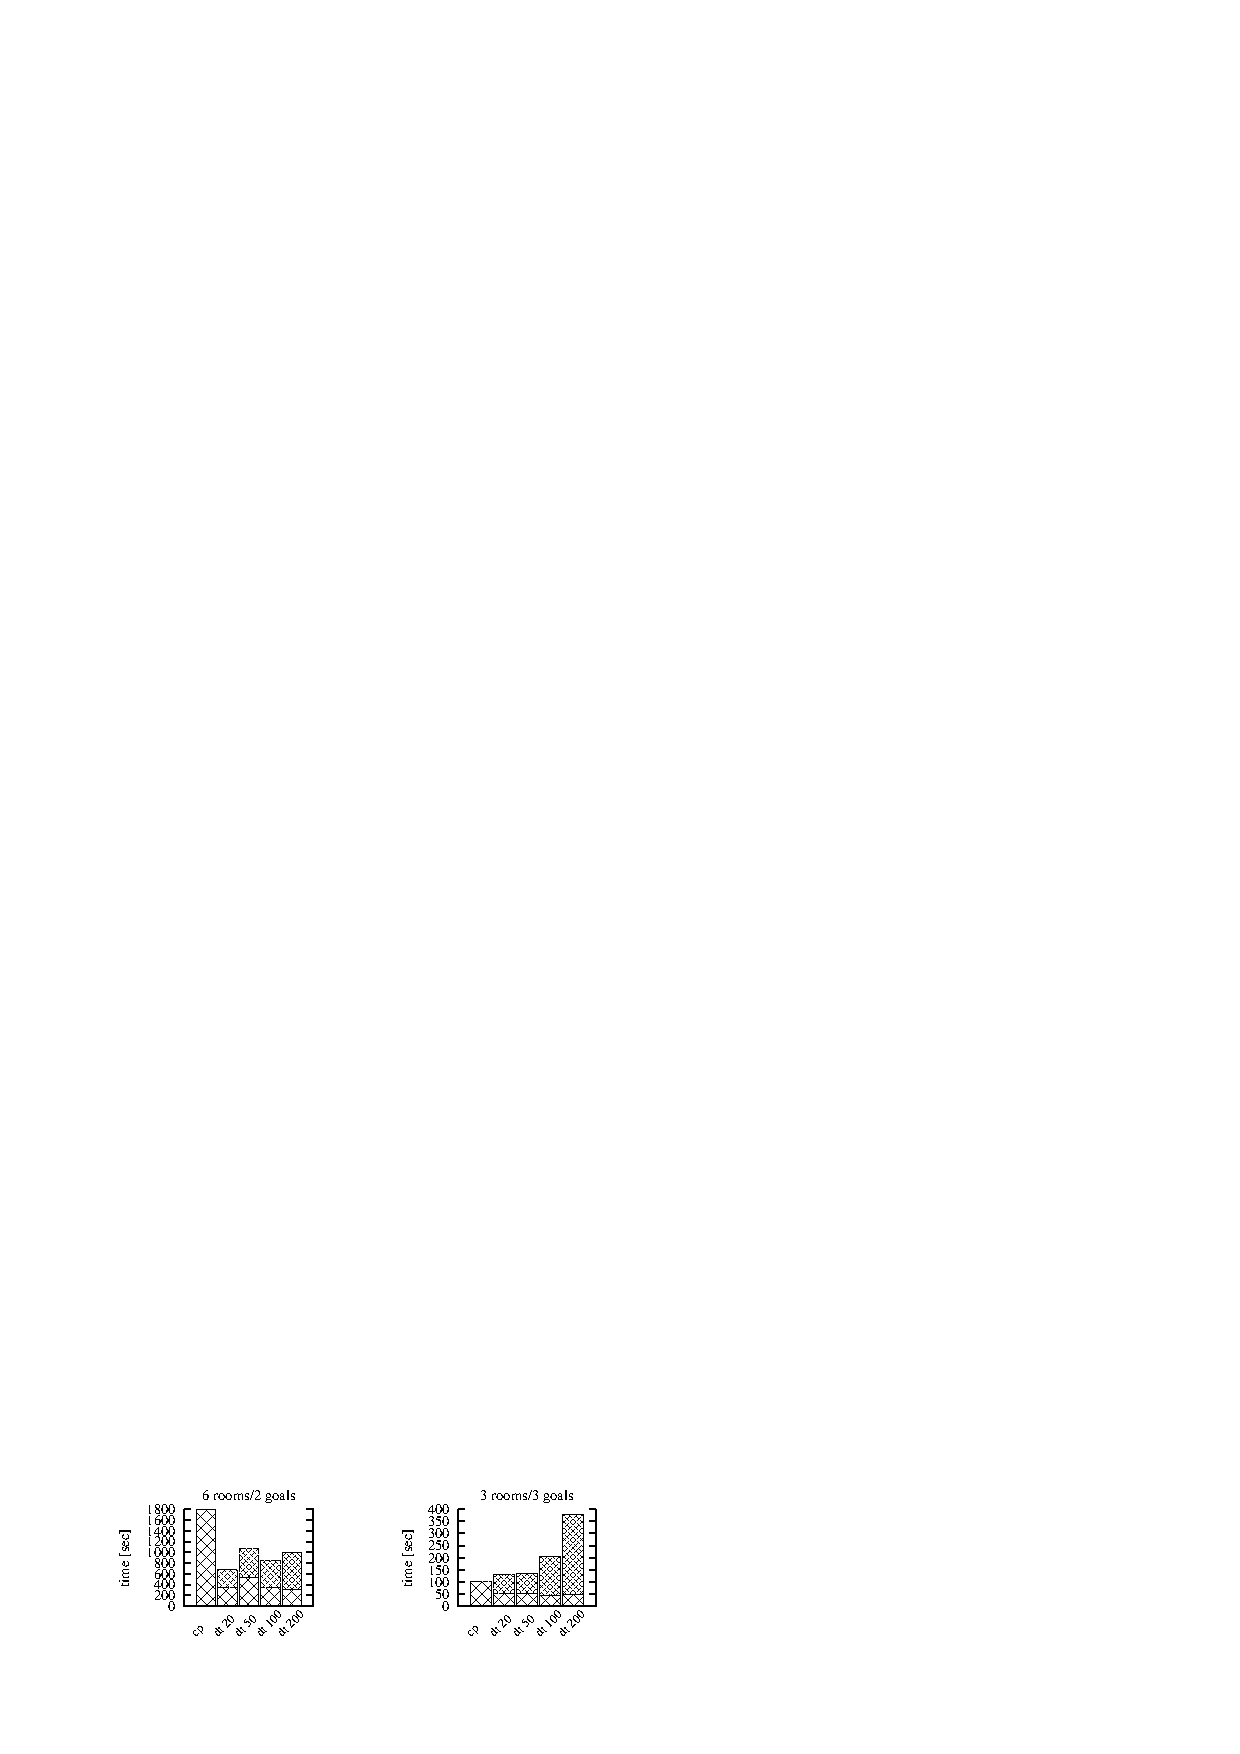
\includegraphics{dora56-time}\hfill
  % \vspace{2mm}
  % 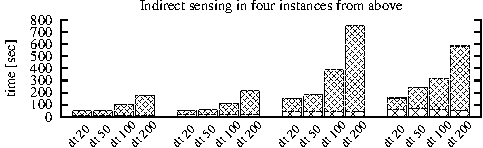
\includegraphics{dora-cat-time}\hfill
  \caption{Average runtime}
  \label{fig:results-time}
\end{figure}

\begin{figure}[h!]
  % \centering
  % 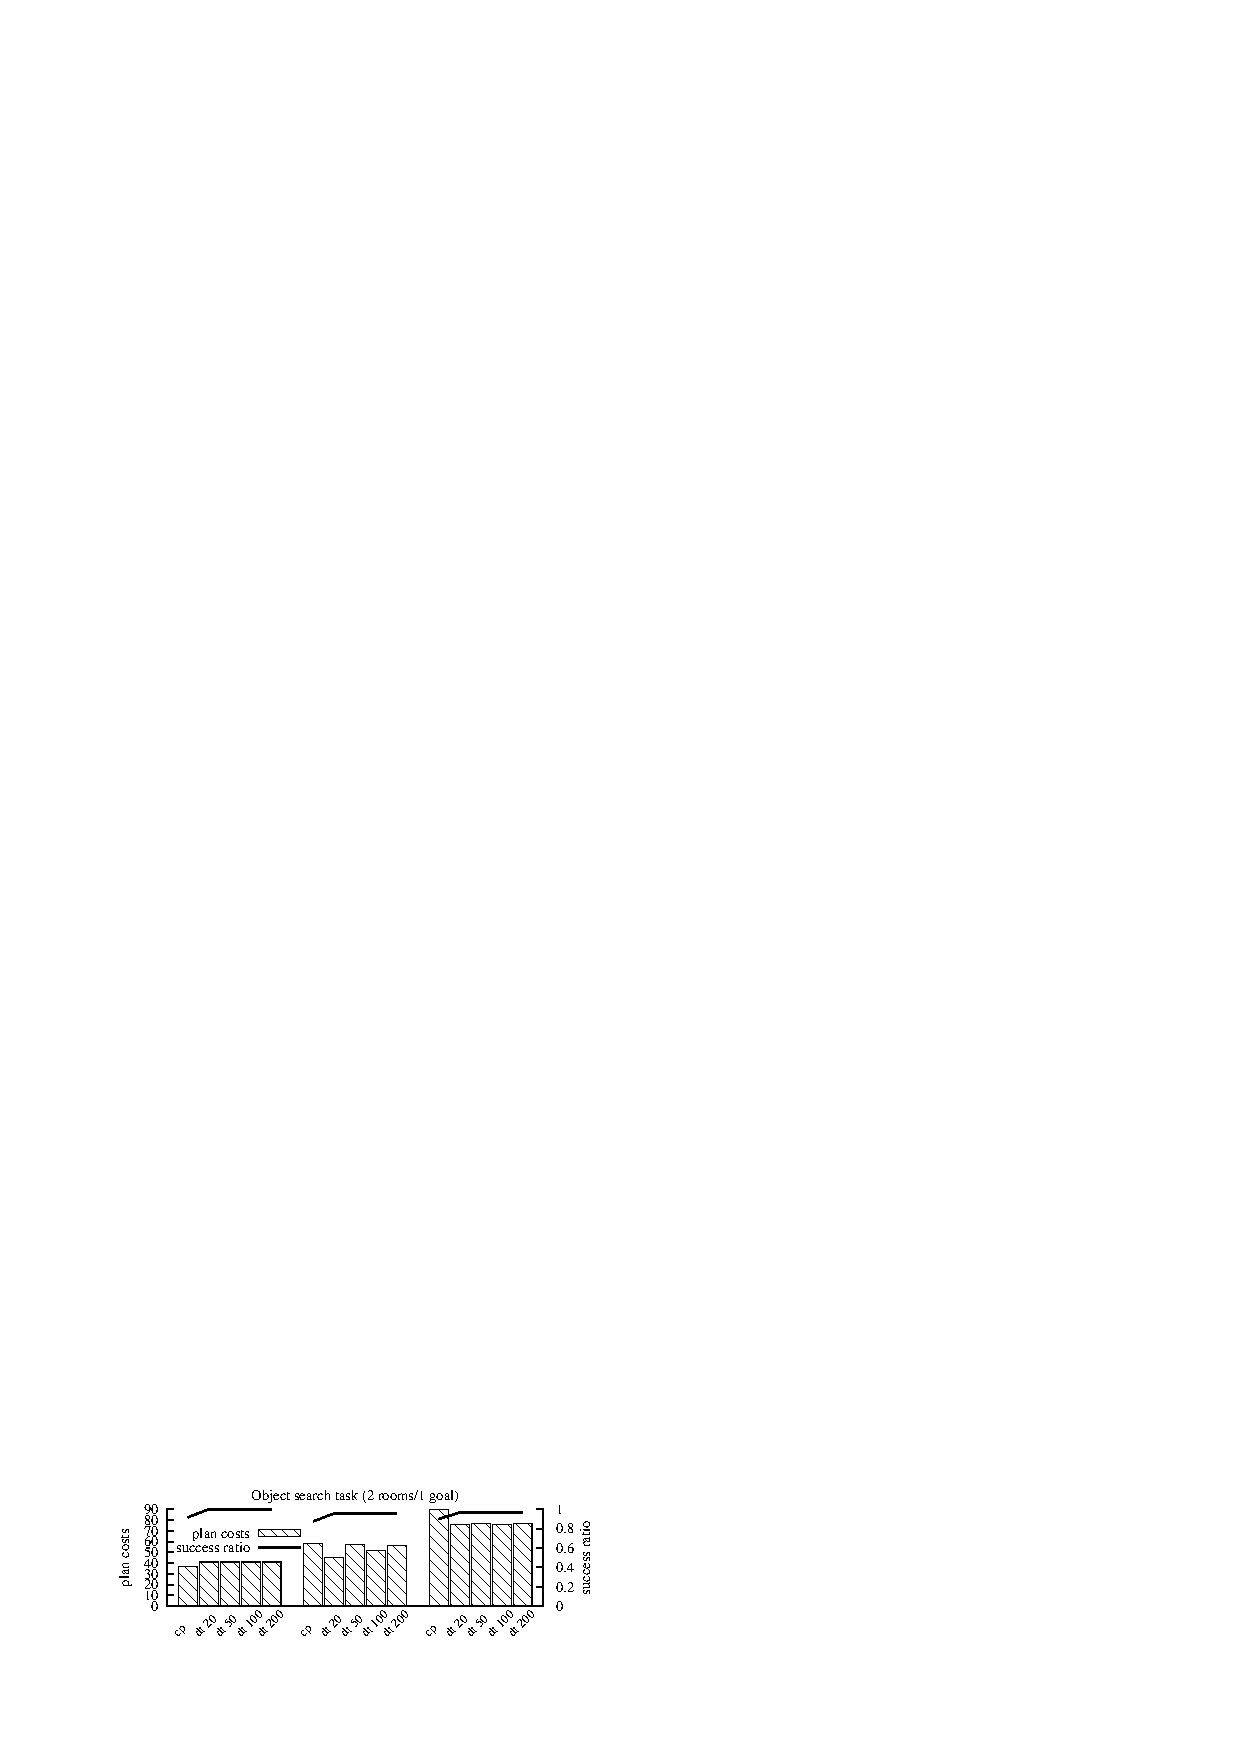
\includegraphics{dora1-quality}\hfill
  % \vspace{2mm}
  % 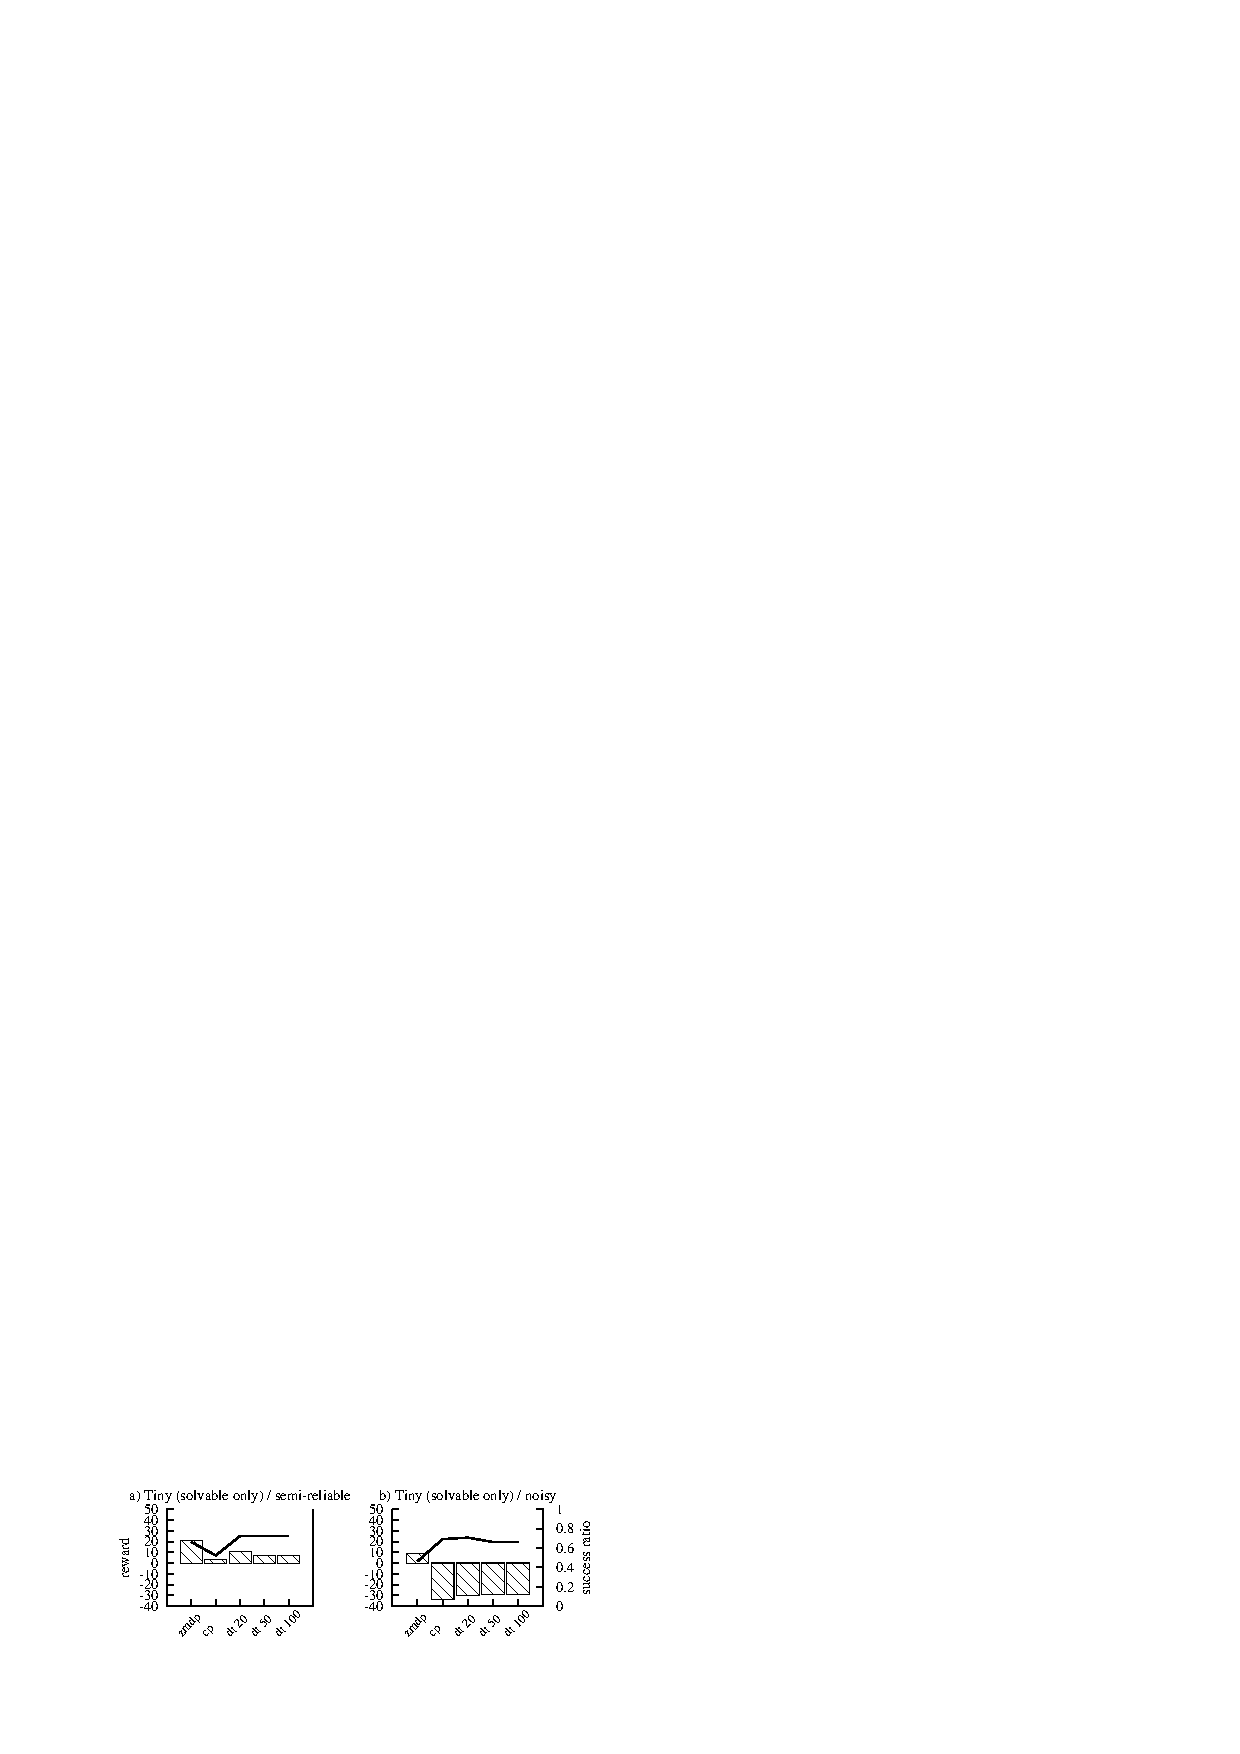
\includegraphics{pomdp-solvable-quality}\hfill
  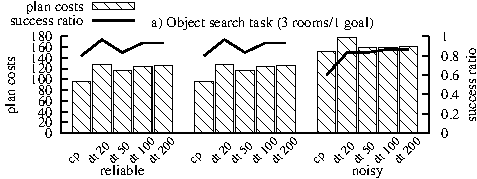
\includegraphics{dora2-quality}\hfill
  % \vspace{2mm}
  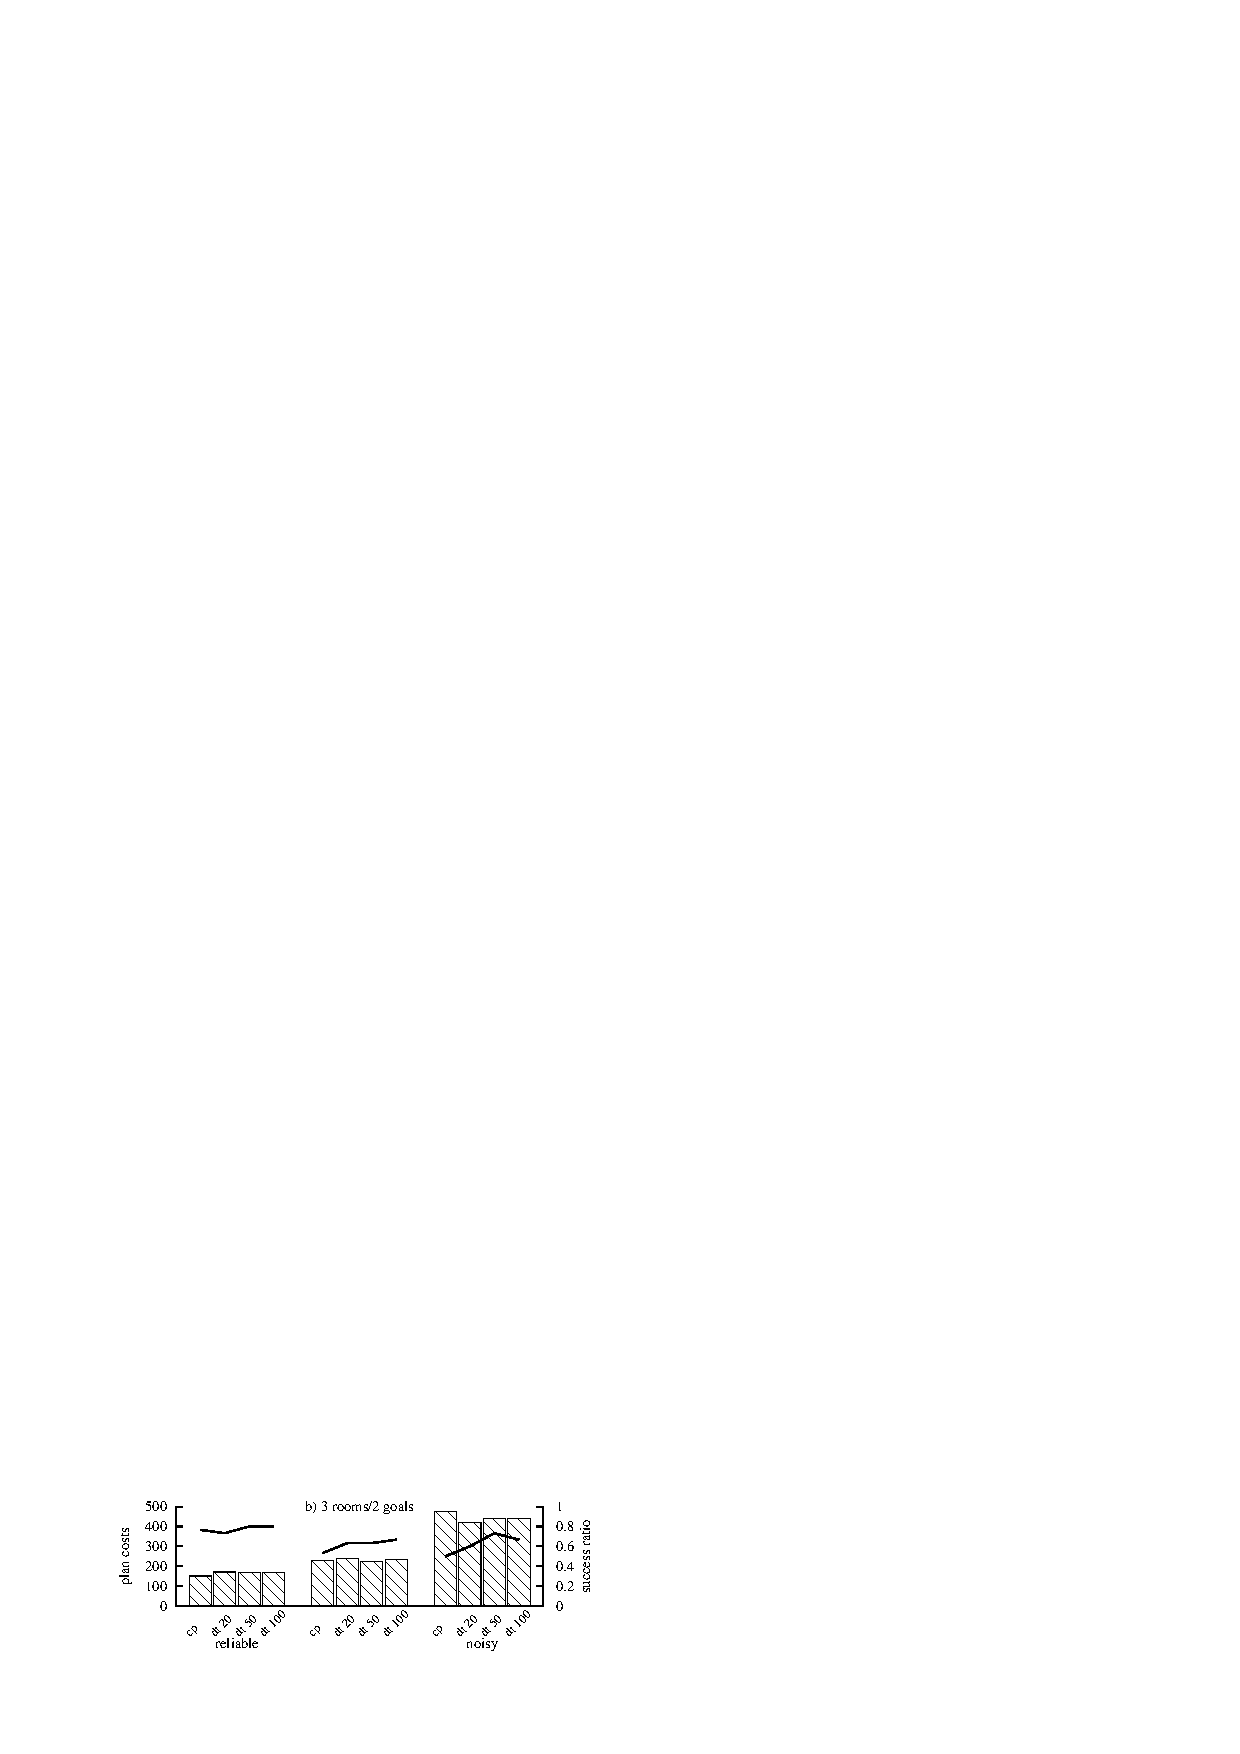
\includegraphics{dora3-quality}\hfill
  % \vspace{2mm}
  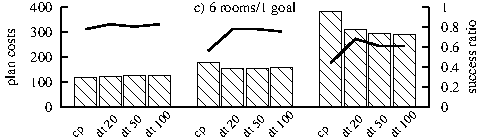
\includegraphics{dora4-quality}\hfill
  \vspace{2mm}
  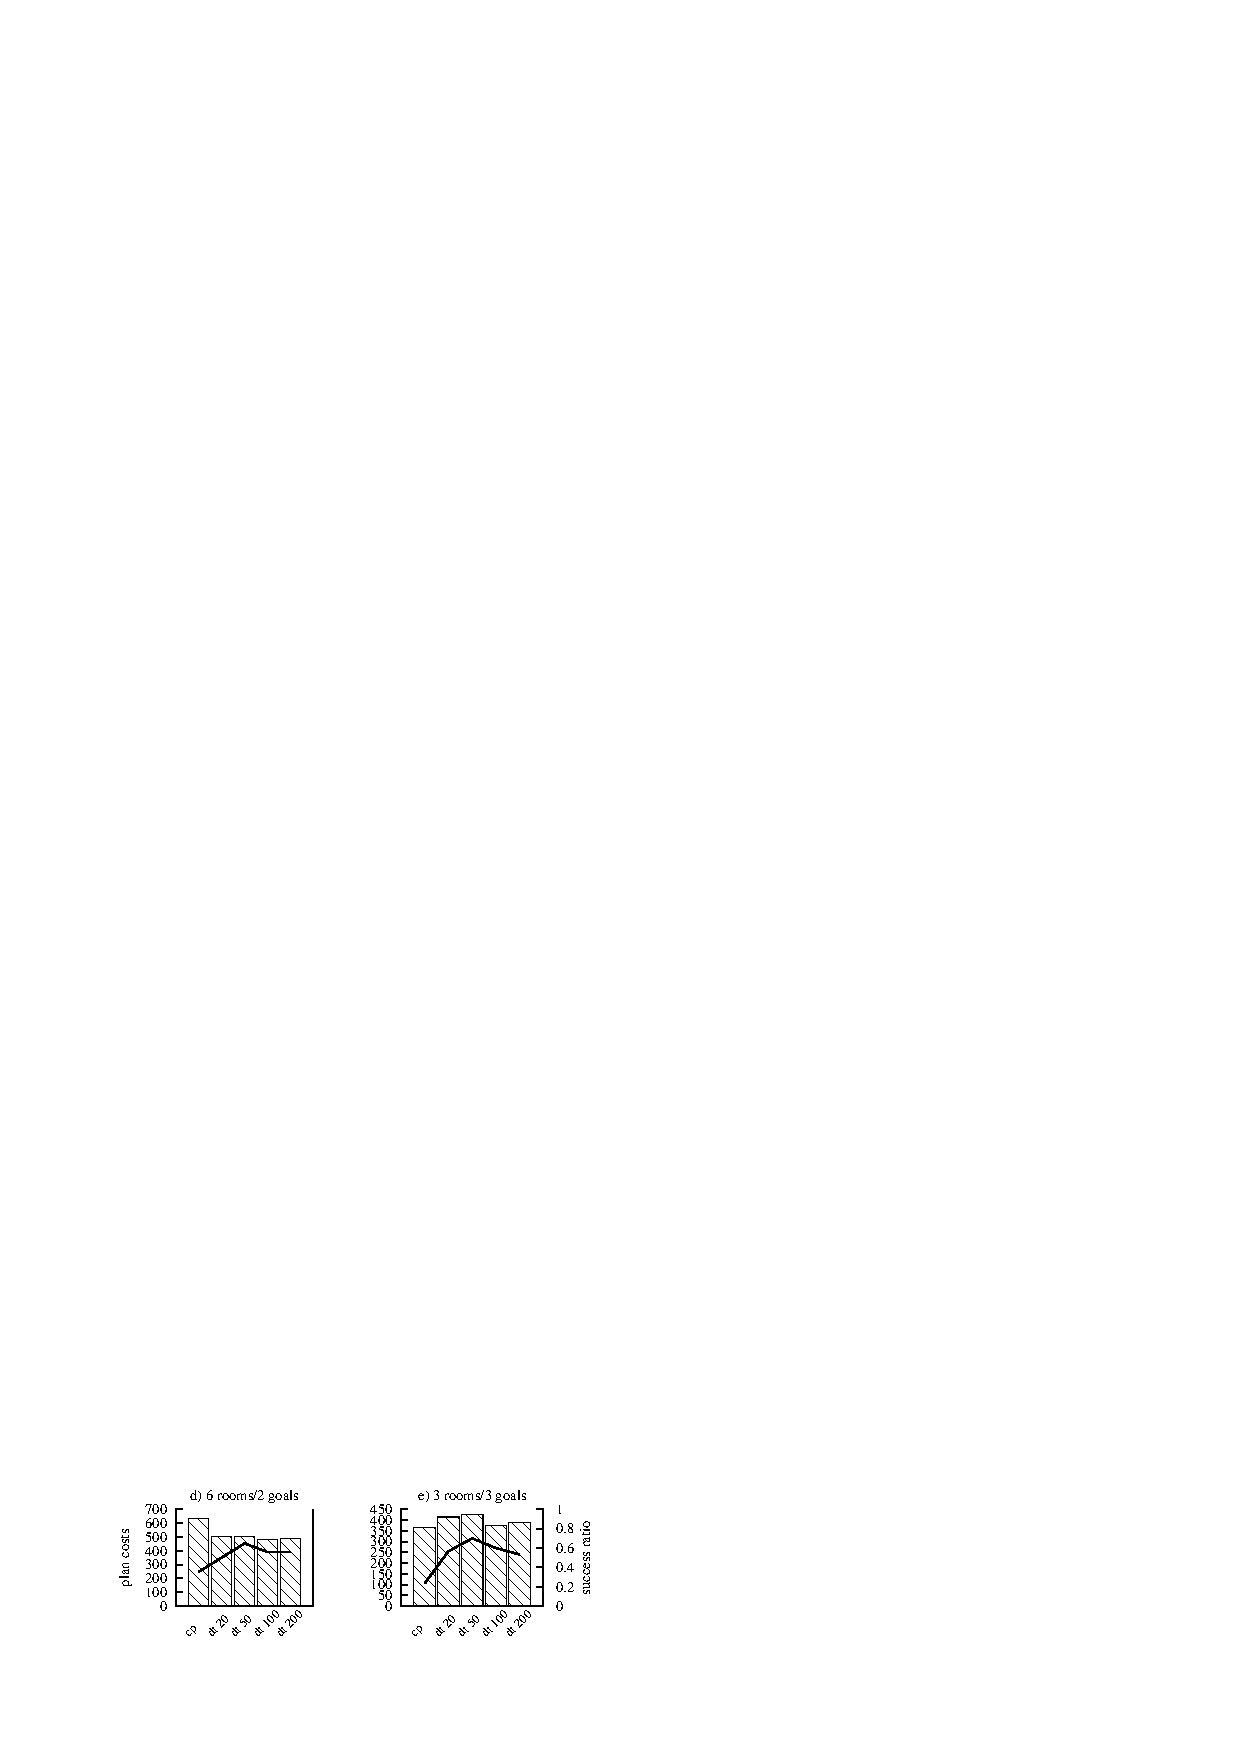
\includegraphics{dora56-quality}\hfill
  \vspace{2mm}
  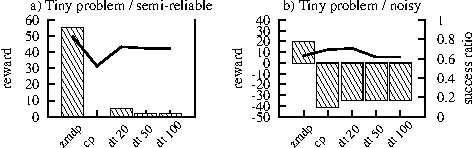
\includegraphics{pomdp-quality}\hfill
  % \vspace{2mm}
  % 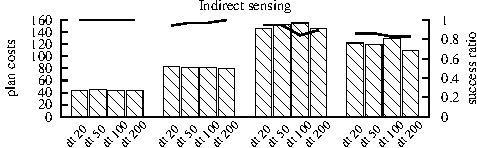
\includegraphics{dora-cat-quality}\hfill
  \caption{Average plan costs and number of successful runs.}
  \label{fig:results-quality}
\end{figure}

We find that if sensing is reliable, then little is gained using DT
sessions, as the greedy approach of the baseline is
sufficient. As sensing degrades DT sessions prove more useful. Here,
time spent on DT planning increases steeply as the abstraction becomes
more refined, which is compensated for by fewer planning sessions
overall. More detailed abstractions lead to a better overall
success rate, particularly for tasks $d$ and $e$.
%% Moreover,
%% for less refined abstractions, the increased cost of DT planning is
%% partially compensated for by a decrease in Fast Downward planning
%% times. 
Speaking to the effectiveness of our entropy heuristic for abstraction
refinement, we see relatively high success rates irrespective of
the level of refinement. Comparing finally to the best {\sc
zmdp} policy, although producing relatively costly plans, the
continual planners performed quite well, especially in terms success
rate. A key source of inefficiency here, is due to sequential sessions
always being optimistic, and refusing to abandon the search.

%%% Local Variables: 
%%% mode: latex
%%% TeX-master: "aaai11"
%%% End: 
